% !TEX root = ../main.tex
\subsubsection{Electron Variables}
\label{14.21::electron_variables}
    First, we'll study the $Q^2$ and $\nu$ acceptances for the scattered $e^-$.
    $Q^2$ and $\nu$ acceptances are presented in Figure \ref{fig::14.21::electron_acc}.
    Each one is presented in integrated kinematical region for the other variable.

    \begin{figure}
        \centering
        % Q2.
        \begin{subfigure}[b]{0.49\textwidth}
            \centering
            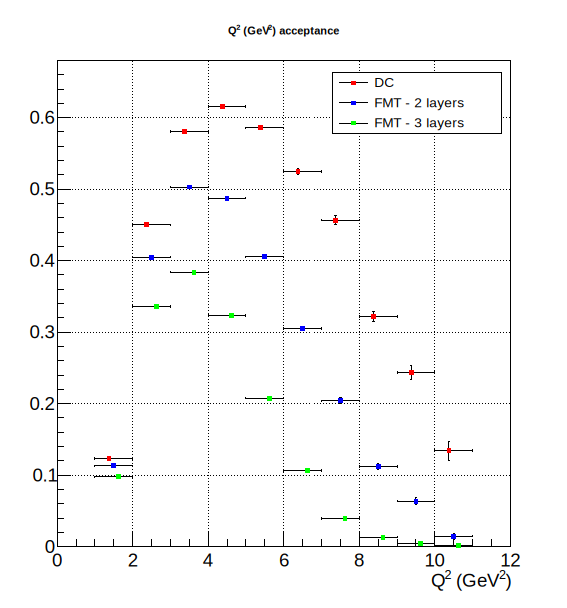
\includegraphics[width=\textwidth]{21q2_acc.pdf}
            \caption{$Q^2$ acceptance.}
            \label{fig::14.21::q2_acc}
        \end{subfigure}
        \hfill
        % nu.
        \begin{subfigure}[b]{0.49\textwidth}
            \centering
            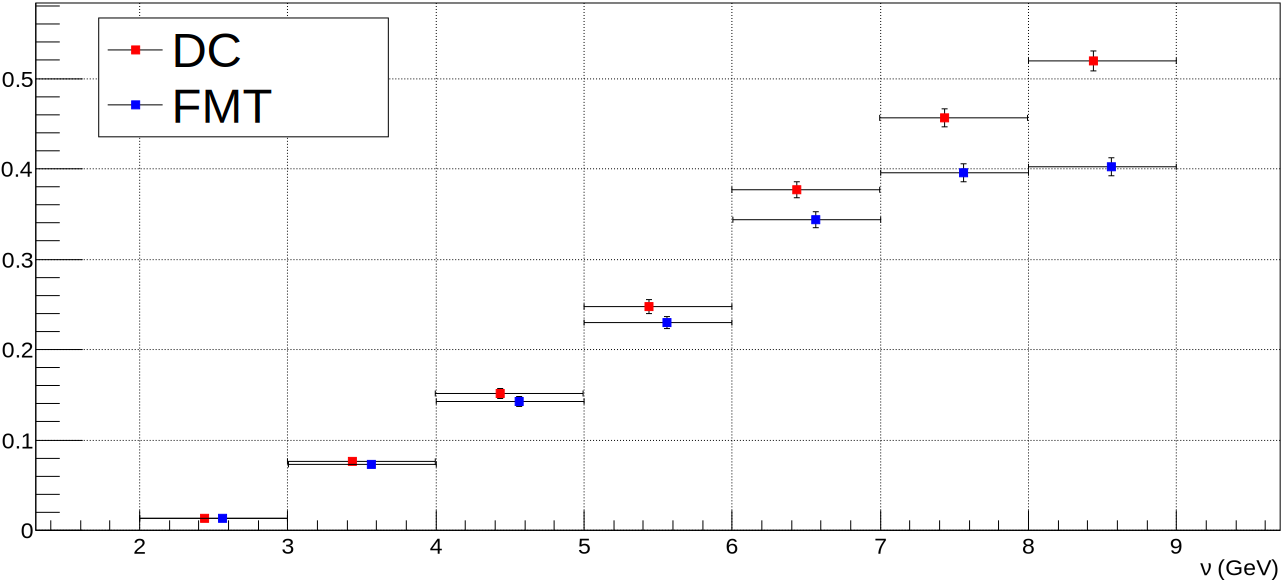
\includegraphics[width=\textwidth]{21nu_acc.pdf}
            \caption{$\nu$ acceptance.}
            \label{fig::14.21::nu_acc}
        \end{subfigure}
        \caption[Electron variables acceptance.]{Electron variables acceptance. $\nu$ is integrated in \ref{fig::14.21::q2_acc}, and $Q^2$ is integrated in \ref{fig::14.21::nu_acc}.}
        \label{fig::14.21::electron_acc}
    \end{figure}
